\section{Results \& Evaluation}\label{results}


\subsection{Evaluation Process}

During the iterative process of designing the interfaces, before they were finalised, the project supervisor helped make styling decisions.

In order to correctly evaluate the interface design, a survey was performed on participants specifically from University of Strathclyde in the Computer Science department. The demographic ranged from Students to Lecturers. No other personal information was collected and any personally identifiable information was redacted.
% TODO: this paragraph previously ended mid-sentence ("Furthermore,") --
% restore the intended continuation if one was planned.

The survey as of \emph{18 July 2026} settled on 24 participants.

Unfortunately, a functional assessment where end-users tangibly interact with the interfaces was not possible due to time constraints and issues surrounding what happens with the data collected such as GDPR and user consent. The data would be stored on personal drives, which would define the surveyor as liable. 

It was decided it was best to use Qualtrics instead, where the survey contained 8 questions, varying by 2 less if you selected to be declare yourself a student. The removed questions were pertaining to the documentation requirement of this project, which meant they were not applicable to students.

\subsection{Results of Evaluation}
This Section includes a direct interpretation of the gathered data and evaluation processes. Figures~\ref{fig:survey_q1}, \ref{fig:survey_q3} and \ref{fig:survey_q5} summarise the responses to the three interface features shown to participants, with each question broken down by respondent type.

\begin{figure}[H]
    \centering
    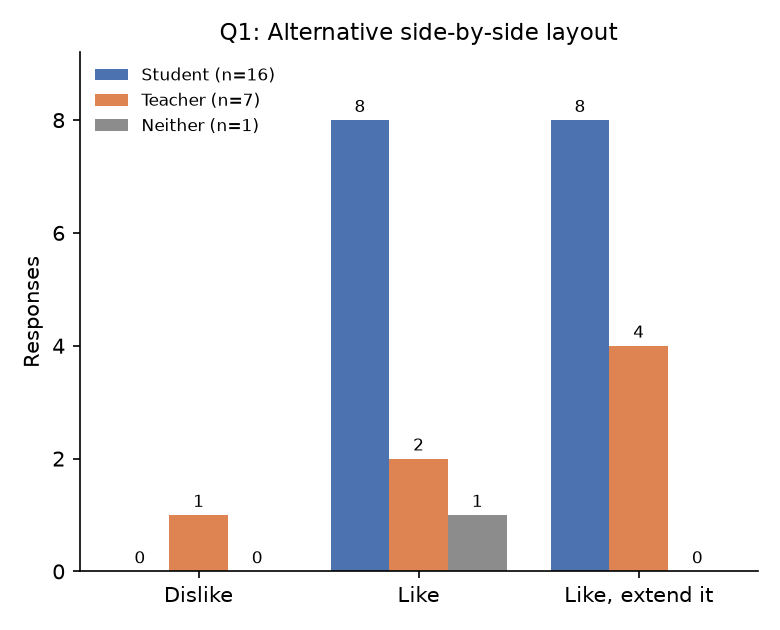
\includegraphics[width=0.7\textwidth]{figs/survey_q1.png}
    \caption{Survey responses to the alternative layout (Q1), broken down by respondent type.}
    \label{fig:survey_q1}
\end{figure}

\begin{figure}[H]
    \centering
    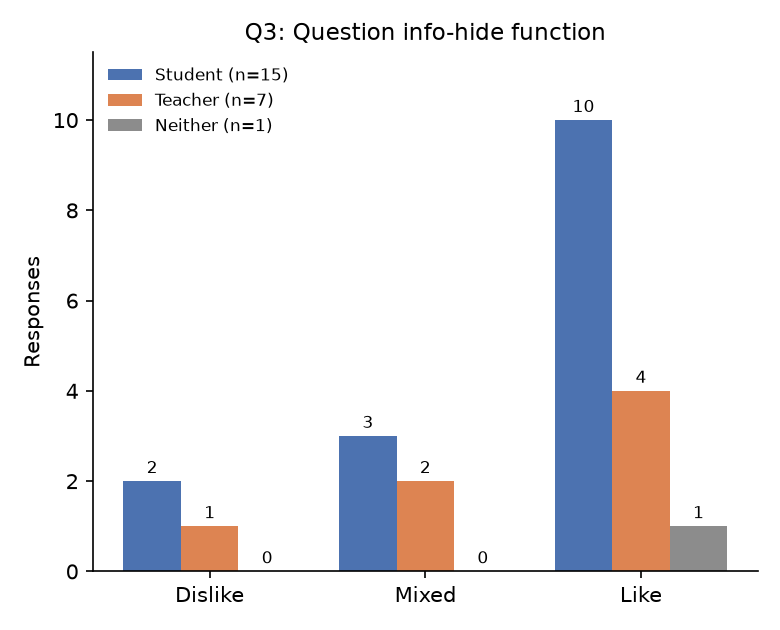
\includegraphics[width=0.7\textwidth]{figs/survey_q3.png}
    \caption{Survey responses to the info-hide function (Q3), broken down by respondent type.}
    \label{fig:survey_q3}
\end{figure}

\begin{figure}[H]
    \centering
    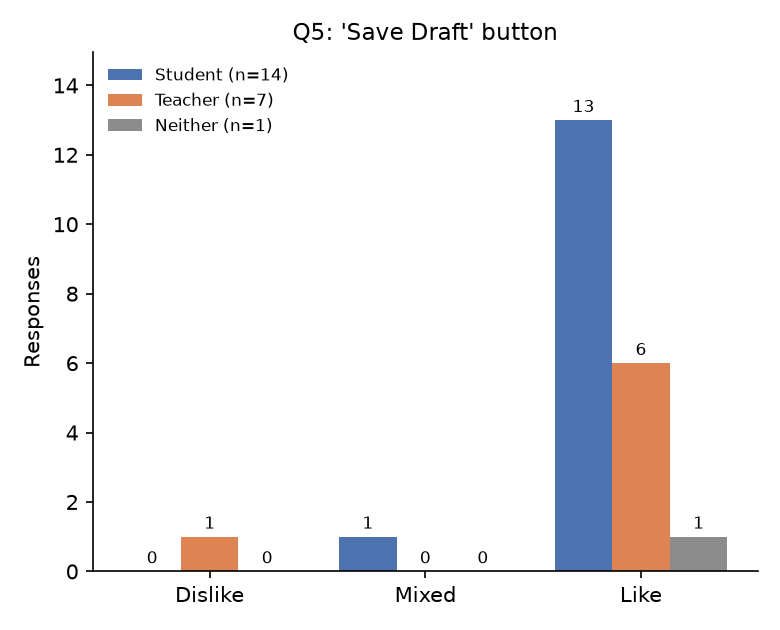
\includegraphics[width=0.7\textwidth]{figs/survey_q5.png}
    \caption{Survey responses to the Save Draft button (Q5), broken down by respondent type.}
    \label{fig:survey_q5}
\end{figure}

\subsubsection{Reception of the Interface Changes}

Reception of the three interface changes was strongly positive across both roles. The alternative side-by-side layout (Figure~\ref{fig:survey_q1}) received the broadest approval: of the 24 responses to the question, 23 (96\%) were positive, and exactly half of all respondents chose the stronger option of liking it and wanting it implemented on other question types. That second figure is notable because it asks for more than FR7 ever specified; extending the layout switcher beyond CodeRunner questions is therefore recorded as future work. The single negative response came from a teacher.

The info-hide function (Figure~\ref{fig:survey_q3}) was the most divided of the three: 15 of 23 responses (65\%) liked it as delivered, 5 (22\%) judged it a good idea if improved, and 3 (13\%) disliked it. This spread is consistent with the feature being the most novel of the three, since it changes how the page itself behaves rather than adding a discrete control. A majority of both students and teachers still approved, and the appetite for refinement points to polishing the interaction rather than removing it.

The Save Draft button (Figure~\ref{fig:survey_q5}) drew the highest approval rate: 20 of 22 responses (91\%) liked it outright, with one response in each of the remaining categories. The result is striking for a control that was styled to be deliberately unobtrusive, and it confirms that students value reassurance that their work is safe. That the button was afterwards removed does not diminish this finding: the approval attaches to the reassurance, not to the button, and the reassurance is better delivered silently by Moodle's own autosave than by a control that had come to demand explanation and attention of its own. The reasoning behind the reversal is set out in the reflection.

Taken together, the survey substantiates the claim that the features it evaluated were worth building: every feature achieved majority approval within both the student and the teacher group, and no feature was rejected by either group.

\subsubsection{Documentation Findings}

The two documentation questions were shown only to non-student respondents, as they concern authoring rather than answering. Seven teachers responded; five of the answers were substantive, and two were test entries which are excluded from the analysis.

On the current state of CodeRunner's documentation, the responses corroborate the assessment made in Section~\ref{process}. Its quality was acknowledged while its form was criticised: `good, but monolithic and hard to search' and `okay, but not always the easiest to understand'. Two responses located the working knowledge outside the manual altogether, one noting that `a lot of the useful stuff is within the forums and needs a bit of searching to find', and another reporting that they had not consulted the documentation since 2021, preferring to work from third-party examples. One respondent summarised the problem in the words quoted in the Design section: the best way to learn CodeRunner today is to have someone who already knows it explain it.

On the proposed alternative, documentation organised around the author form with contextual explanations, four of the five substantive responses were supportive, ranging from `sounds good' to `plenty of other areas use a similar approach so it seems like a no-brainer' and `this would be useful to stop you needing to look it up'. The remaining response raised a considered governance concern rather than an objection: if authors can contribute to the documentation, someone must hold authority over debatable contributions, and clarity should be valued above concision. These points target the future contribution model rather than the documentation page delivered by this project, and they are recorded as considerations for any community-editable extension of it.

These findings validate the direction taken for NFR3: the criticisms of the existing manual match the deficiencies identified in the analysis, and the approach built in response was endorsed by four of the five substantive teacher responses.

\subsubsection{Evaluation Against the Objectives}
The survey speaks directly to the three interface changes it showed, but the project's objectives are broader, and each carries its own evidence. Objective~1, a reproducible, regression-testable environment, is demonstrated by the two single-command test harnesses and the upstream Behat suite they run (DE1--DE3). Objective~2, the author-page ergonomics, combines the survey's endorsement of the layout and information-panel behaviour with the Behat and manual verification of test-case management (FR1) and the Precheck fix (FR4), and with the measured accessibility gain from 93\% to 97\% (NFR2). Objective~3, the student experience, is precisely what the survey assessed: the alternative layout and the info-hide function each won majority approval in both respondent groups, as did the save-draft button that was subsequently removed for the reasons set out in the reflection. Objective~4, task-focused documentation reachable from the tool, is supported by the four of five substantive teacher responses endorsing the approach and by the delivered page, its editing-form link and its search. Objective~5, evaluating the changes with real users to derive further requirements, is discharged by the survey itself, which both validated the delivered work and produced the future-work items discussed in the reflection that follows. The three deferred requirements (FR3, FR5 and FR9) leave acknowledged gaps within the second and third objectives, but no objective is left unmet and no delivered feature was judged unwanted by either audience.

